\documentclass{usireport}

%% VARIABLES
\newcommand\namesurname{Alessandro Gobbetti}
\newcommand\assignment{Assignment 1}
\newcommand\assignmenttitle{}

\newcommand\subject{Mobile and Wearable Computing}

\begin{document}
\maketitlepage

\section{Introduction}
This is the first assignment for the Mobile and Wearable Computing course. The goal is to get familiar with Android development by updating an existing application and answering questions about Android components and UI elements. 

The code is available at: \url{https://github.com/Alessandro-Gobbetti/Mobile-and-Wearable-Computing}.

\section{Exercise 1: Update the StepAppV1 application}

The StepApp application developed during the tutorial was a simple step counter that displayed the number of steps, a button to increment the step count (see \autoref{fig:stepapp_count}), and a button that displayed a toast message when pressed (see \autoref{fig:stepapp_start}). The goal of this exercise was to update the StepApp application so that when the user presses the start button, the step count is reset to zero.


\begin{figure}[H]
    \centering
    \begin{subfigure}{0.4\textwidth}
        \centering
        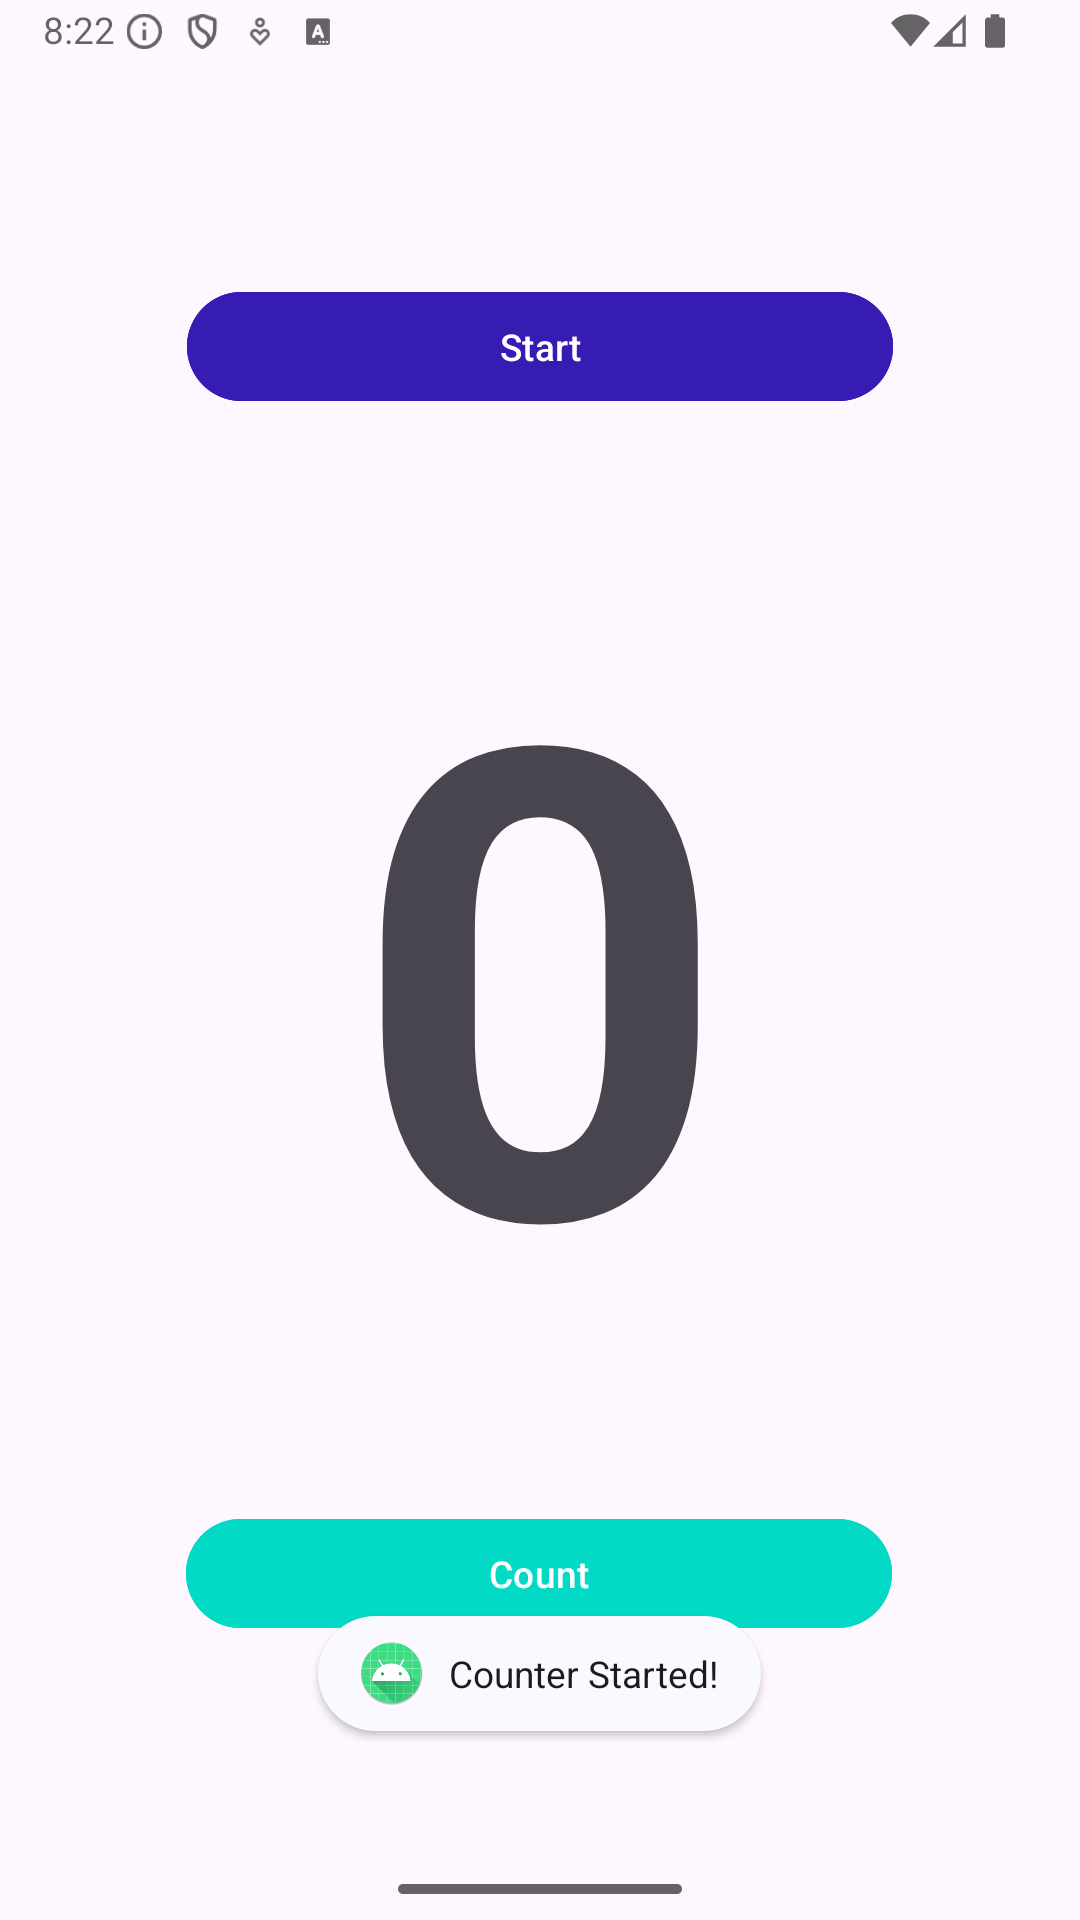
\includegraphics[width=0.63\linewidth]{fig/stepapp_start.png}
        \caption{StepApp after pressing the start button}
        \label{fig:stepapp_start}
    \end{subfigure}
    \hspace{1cm}
    \begin{subfigure}{0.4\textwidth}
        \centering
        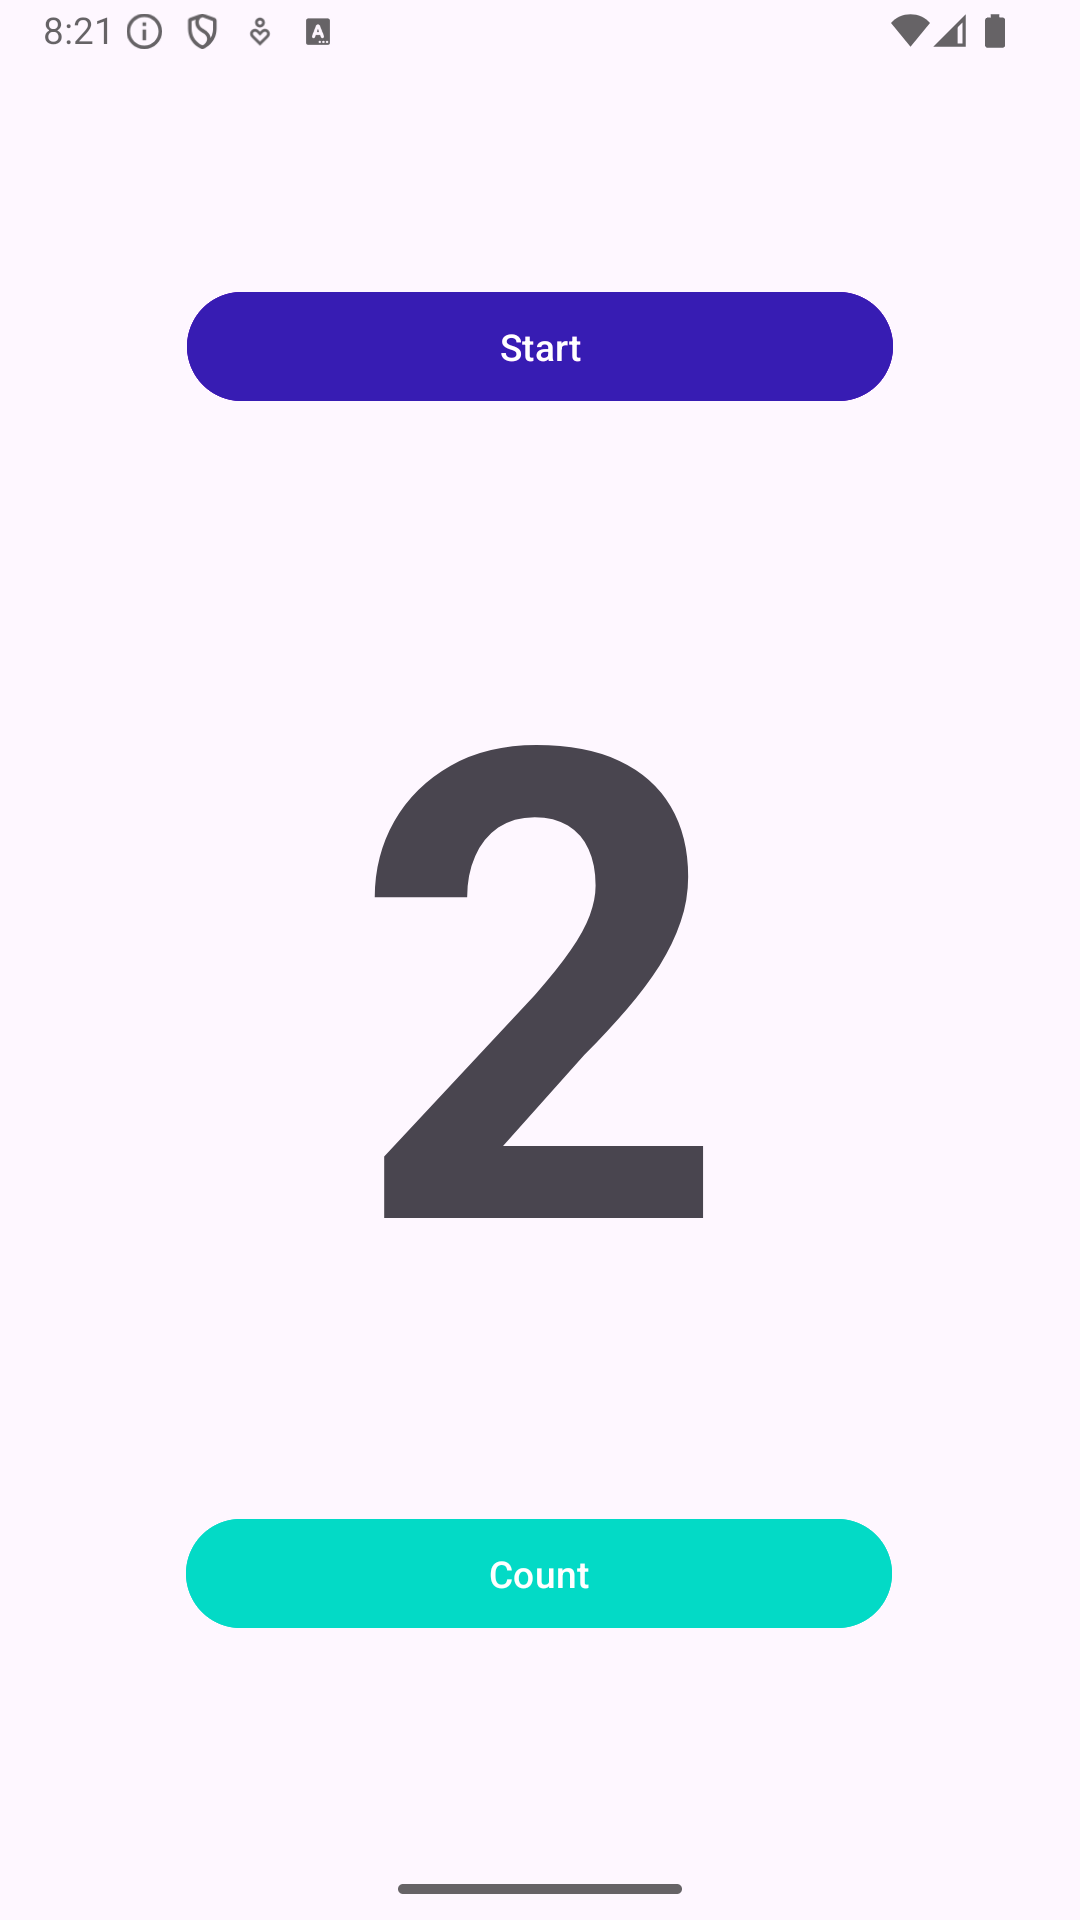
\includegraphics[width=0.63\linewidth]{fig/stepapp_count.png}
        \caption{StepApp while counting}
        \label{fig:stepapp_count}
    \end{subfigure}
    \caption{StepApp}
    \label{fig:stepapp}
\end{figure}


As shown in the code below, the \mintinline{java}{startCount} method executed when the start button is pressed not only displays a toast message but also resets the \mintinline{java}{stepCounter} variable to zero and updates the view to display the new count.

\begin{minted}{java} 
public class MainActivity extends AppCompatActivity {

    private int stepCounter = 0;
    private TextView showCount;

    ...

    public void startCount(View view) {
        Toast toast = Toast.makeText(this, R.string.counterStarted, Toast.LENGTH_LONG);
        toast.show();

        // Reset the counter
        stepCounter = 0;
        // update the view
        showCount.setText(String.valueOf(stepCounter));
    }
    ...
}
\end{minted}


\section{Exercise 2}

\textbf{Question 1:} Describe briefly the four components of Android application, use an application example similar to the Twitter application example in T01 to demonstrate your answer.

\textbf{Answer:} The four components of an Android application are: Activities, Services, Broadcast Receivers, and Content Providers. 

Activities are the visible components, they are single screens of the application allowing the user to interact with it. They can be reused across different applications. For example in a fitness-tracking app, the main screen where the user can see their daily step count, calories burned, and distance traveled is an Activity. If the user wants to see their weekly progress, they can navigate to a different Activity that shows a graph of their weekly step count.

Services are background components that perform long-running operations without a user interface. The fitness-tracking app could have a Service that runs in the background and traks the users' steps and location throughout the day. The service ensures that that the app stays operational even when the user is not actively using it.

Broadcast Receivers wait for system-wide events to occur, such as a low battery warning or a new SMS message. The fitness-tracking app could have a Broadcast Receiver that listens for battery level changes. It might alert the user and suggest pausing a workout to save battery or sync data to avoid loss.

Content Providers are interfaces for sharing data between applications. Small pieces of data exchanges are possible via intents but Content Providers are more suitable for larger data sets (such as contacts). The fitness-tracking app could have a Content Provider that allows other apps to access the user's workout data. For example, a nutrition app could use the fitness-tracking app's Content Provider to suggest meal plans based on the user's activity level.

\bigbreak

\textbf{Question 2:} Describe the differences between the View and the ViewGroup UI elements in Android applications. Provide an example for the \mintinline{java}{View} and the \mintinline{java}{ViewGroup} to demonstrate your answer.

\textbf{Answer:} In Android applications, the \mintinline{java}{View} class is the basic building block of the user interface. It represents a single UI element that the user can interact with. Examples of \mintinline{java}{View} elements are buttons, text fields, and images. The \mintinline{java}{View} class is the superclass of all UI elements in Android.
Taking the example from before, the main screen of the fitness-tracking app could have a \mintinline{java}{View} for the step count, another one for the calories burned, one for start/stop button, and so on.

A \mintinline{java}{ViewGroup} is a subclass of \mintinline{java}{View} that can contain multiple \mintinline{java}{View} elements. It is used to arrange and group together the different UI elements for better organization. Layouts are specific types of \mintinline{java}{ViewGroup} used to define the visual structure of the app (e.g., linear layout, relative layout, grid layout, ...). In the fitness-tracking app, the main screen could be a \mintinline{java}{ViewGroup} that contains the \mintinline{java}{View} elements for the step count, calories burned, and other information.

\end{document}





